Ein Teil des Integrationstests ist der Schnittstellentest. Schnittstellen sorgen dafür, dass
Softwareteile, insbesondere Softwarekomponenten miteinander verbunden sind und Daten austauschen können.
Es werden verschiedene Arten von Schnittstellendefinitionen vorgestellt und es wird gezeigt, wie eine 
Schnittstelle getestet werden kann.
In Abbildung 2.1 ist zu sehen, wie zwei Komponenten durch eine Schnittstellendefinition verbunden sind.\par
\begin{figure}[!h]
\centering
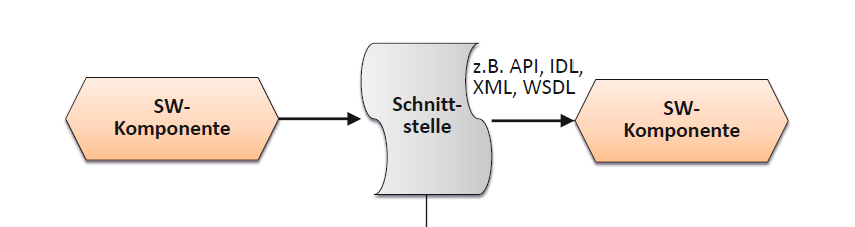
\includegraphics[scale=.9,]{Bilder/Quicktest/Schnittstelle.png}
\caption{Schnittstellen \parencite[S.218]{integration}}\label{fig:schnitt}
\end{figure}
Es gibt verschiedene Arten, wie man eine Schnittstelle definieren kann \parencite[S. 218 ff.]{integration}:
\begin{description}
\item[unstrukturierte Datenübergabe] Es gibt keine feste Schnittstellendefinition. 
Der Empfänger muss die Daten selbst interpretieren. %Automatisierte Analysen sind kaum möglich.
\item[Gemeinsame globale Datenbereiche] Komponenten können darauf zugreifen, Werte ablegen und entnehmen.
Wenn beide Komponenten jedoch eine eigene Definition des Datentyps haben, wird die Wartbarkeit bei Änderungen
schwierig. Abhilfe kann hier eine Header Datei sein, in der die Datenstruktur definiert ist. Eine Header Datei
dient als Schnittstelle zwischen Dateien. Damit können Daten für mehrere Dateien sichtbar gemacht werden.
\item[\ac{api}] Daten werden über eine \ac{api} übertragen. Dabei werden die Daten 
in einen Stapel gespeichert und an die Zielkomponente übergeben, welche die Daten vom Stapel entpackt. Es kann
ein Rückgabewert (Return) an die Senderkomponente zurückgesendet werden.
%Dateien später bei xml, sql bla bla
\item[Datenbanken] Der Datenaustausch ist über eine gemeinsame Datenbank definiert. Die erste Komponente legt
Daten ab, die zweite Komponente holt die Daten. Datenbanken
werden oft in IT-Systemen eingesetzt.
Der Test einer Datenbank kann erfolgen, indem Dateninhalte überprüft werden. Es bietet sich auch an, die Datenbank
zu manipulieren, indem einzelne Zeilen oder Spalten verändert werden, um die Auswirkungen zu überprüfen.
\item[Schnittstellendefinitionssprachen] Sie haben die Aufgabe eine sichere Datenübertragung
zu ermöglichen, indem die Struktur der zu sendenden Daten klar definiert wird.
Eine Schnittstellendefinitionssprache ist \ac{xml}. In einem Schema wird die 
Struktur und der Inhalt der Schnittstelle festgelegt. Anhand dieses Schemas wird überprüft, ob die Daten richtig sind.
Ein Vorteil von \ac{xml} ist, dass es einfach erweiterbar ist. Es ist auch sehr flexibel, sodass eine Schema nach
den eigenen Bedingungen erstellt werden kann. Es ist sinnvoll, strenge Regeln aufzustellen, damit eine Überprüfung besser
möglich ist.
\end{description}


\section*{Schnittstellentest}
Für den Schnittstellentest benötigt es zwei Schritte, wie in Abbildung 2.2 zu sehen ist.
Ein Schritt ist, dass getestet wird, ob das Format der Schnittstellendefinition eingehalten wird.
Ein Entwickler schreibt die Schnittstelle und die Überprüfung erfolgt von einer zweiten Person. Der Überprüfer hat einen
anderen Blickwinkel und kann Denkfehler besser erkennen und sofort lösen \parencite[S. 226]{integration}.
Als Beispiel einer Schnittstelle wird im Folgenden \ac{xml} genommen.
Es gibt automatisierte Tests wie einen XML-Analysator. Dieser überprüft XML-Daten gegen die Struktur im vorgegebenen
Schema \parencite[S. 237]{integration}.

Damit werden nur die XML-Daten an sich überprüft. Ein zweiter wichtiger Punkt ist die Überprüfung des Zugriffs auf die Daten, die in einer XML hinterlegt sind.
Dafür muss der Code geprüft werden, in der die Schnittstelle verwendet wird.
Die Schnittstelle wird auf Empfänger- und Senderseite überprüft. Dabei können Parameter wie der Typ, die Reihenfolge oder die Nutzungsart eine Rolle spielen \parencite[S. 228]{integration}.\par
\begin{figure}[!h]
\centering
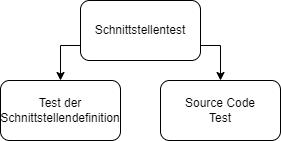
\includegraphics[scale=.9,]{Bilder/Quicktest/Schnittstellen.drawio.png}
\caption{Schnittstellentest \parencite[S. 226]{integration}}
\end{figure}














% Die Schnittstelle wird auf den Typ, die Reihenfolge, die Nutzungsart
% % die Parameter der Schnittstellendefinition, den Typ, die Reihenfolge, die Nutzungsart
% mit den Ein-/Ausgabe-Operationen geprüft.

 % Die Schnittstelle soll gelesen und geprüft werden.
% Es kann ein sogenanntes Review machen. Einer  
% Dies kann mit einem XML-Analysator überprüft werden. 
% Ein zweiter Schritt ist, dass der Source Code getestet wird, ob diese Schnittstelle richtig angewandt wird.\par


% die Schnittstellendefinition überprüft werden.
% Zum Anderen muss der Source Code überprüft werden, ob diese Schnittstelle richtig gemacht wird.
% Bild: Test Schnittstellen 
% Überprüfung Schnittstellendefinition, zweiter Punkt Abgleich (Baustein A, Baustein B) Seite 226

% Beim Abgleich:
% Informationen aus xml.
% Code wird überprüft, ob Informationen aus xml im Code richtig geschrieben wurden.
% "wird der Source Code der Schnittstelle gelesen und geprüft, ob die Parameter der Schnittstellen-
% definition in der Anzahl, im Typ, in der Reihenfolge und in der Nutzungsart mit den
% Ein/Ausgabe Operationen der Sender und Empfänger der Schnittstelle übereinstimmen"(dh ob die Daten, die in der
% xml über die Schnittstelle definiert wurden, im Code richtig eingesetzt wurden.)

% Bei ZF ist es so:
% Schnittstellen inklusive Signale in xml.
% Code in C geschrieben: Verbindung von zwei Signalen in C Code geschrieben, durch Einsetzen der Makros
% Makros, Header Dateien aus xml generiert.

% Quicktest bei ZF:(das ist genau dieser Abgleich)
% Überprüfen, ob der per Hand geschriebene C Code die Schnittstelle, so wie sie in xml definiert ist,
% richtig abbildet.

% dann zu beiden Punkten noch was schreiben





% 12.1.x aufzählen
% Schnittstellen Review

% Bild auf Seite 231 ist auch gut.
% 12.2 Ansätze für Tests ab Seite 225

% eine Lösung ist statische Schnittstellenanalyse